\chapter{The Loss Function: Binary Cross Entropy}
\label{chap:log_loss}

% ========================================
% SECTION 1: WHY NOT MSE?
% ========================================
\section{Why Not Mean Squared Error (MSE)?}
In Linear Regression, we used MSE as the loss function. Can we use it for Logistic Regression?
\begin{equation}
    J = \frac{1}{n} \sum (\sigma(z) - y)^2
\end{equation}
The answer is \textbf{No}. If you plot this loss function against the weights ($w$), it turns out to be \textbf{Non-Convex}.

\begin{itemize}
    \item It has many ``local minima'' (shallow valleys).
    \item Gradient Descent might get stuck in a local minimum instead of finding the global best solution.
\end{itemize}

\begin{figure}[htbp]
\centering
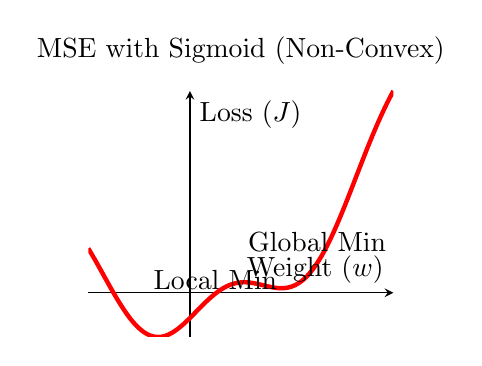
\begin{tikzpicture}
    \begin{axis}[
        xlabel={Weight ($w$)},
        ylabel={Loss ($J$)},
        ticks=none,
        axis lines=middle,
        width=0.45\textwidth,
        title={MSE with Sigmoid (Non-Convex)}
    ]
    \addplot[domain=-2:4, samples=100, smooth, ultra thick, color=red] {sin(deg(x*2)) + 0.5*x^2 - 1};
    \node at (axis cs:0.5, 0.5) {Local Min};
    \node at (axis cs:2.5, 2) {Global Min};
    \end{axis}
\end{tikzpicture}
\hfill
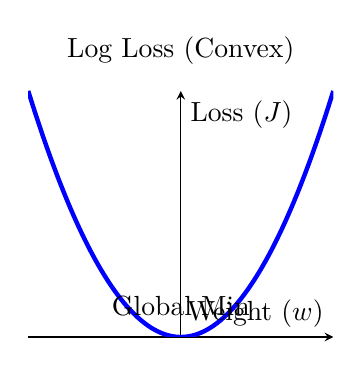
\begin{tikzpicture}
    \begin{axis}[
        xlabel={Weight ($w$)},
        ylabel={Loss ($J$)},
        ticks=none,
        axis lines=middle,
        width=0.45\textwidth,
        title={Log Loss (Convex)}
    ]
    \addplot[domain=-2:2, samples=100, smooth, ultra thick, color=blue] {x^2};
    \node at (axis cs:0, 0.5) {Global Min};
    \end{axis}
\end{tikzpicture}
\caption{Non-Convex (MSE) vs Convex (Log Loss). Gradient Descent is guaranteed to find the global minimum only for convex functions.}
\label{fig:convexity}
\end{figure}

% ========================================
% SECTION 2: MLE
% ========================================
\section{Maximum Likelihood Estimation (MLE)}
Instead of thinking about ``minimizing error'', we switch to a probabilistic view.

\begin{definition}
\textbf{Maximum Likelihood Estimation (MLE)}: A method to estimate model parameters by finding the values that \textbf{maximize the probability} of observing the given data.
\end{definition}

\textbf{Intuition}:
\begin{itemize}
    \item If a patient has cancer ($y=1$), we want our model to predict $\hat{y}$ close to 1.
    \item If a patient is healthy ($y=0$), we want $\hat{y}$ close to 0.
\end{itemize}

The \textbf{Likelihood} is the product of individual probabilities:
$$ L = \prod_{i=1}^{n} P(y_i | x_i; w) $$

\textbf{Problem}: Multiplying many small numbers ($0.9 \times 0.8 \times 0.7 \ldots$) leads to numerical underflow.

\textbf{Solution}: Take the \textbf{Logarithm}. Since $\log$ is monotonic, maximizing $\log(L)$ is equivalent to maximizing $L$.
$$ \log L = \sum_{i=1}^{n} \log P(y_i | x_i; w) $$

% ========================================
% SECTION 3: LOG LOSS
% ========================================
\section{Binary Cross Entropy (Log Loss)}
Since we want a \textbf{Loss Function} (to minimize), we take the \textbf{Negative} of the Log Likelihood.

\begin{definition}
\textbf{Binary Cross Entropy} (Log Loss):
\begin{equation}
    J(w) = - \frac{1}{n} \sum_{i=1}^{n} [ y_i \log(\hat{y}_i) + (1-y_i) \log(1 - \hat{y}_i) ]
\end{equation}
\end{definition}

\textbf{How it works}:
\begin{itemize}
    \item \textbf{Case 1: Actual $y = 1$}. The second term vanishes. Loss = $-\log(\hat{y})$.
        \begin{itemize}
            \item If $\hat{y} \approx 1$ (Correct): $-\log(1) = 0$ (No penalty).
            \item If $\hat{y} \approx 0$ (Wrong): $-\log(0) \rightarrow \infty$ (Huge penalty).
        \end{itemize}
    \item \textbf{Case 2: Actual $y = 0$}. The first term vanishes. Loss = $-\log(1-\hat{y})$.
        \begin{itemize}
            \item If $\hat{y} \approx 0$ (Correct): $-\log(1) = 0$.
            \item If $\hat{y} \approx 1$ (Wrong): $-\log(0) \rightarrow \infty$.
        \end{itemize}
\end{itemize}

% ========================================
% SECTION 4: SIGMOID DERIVATIVE
% ========================================
\section{Derivative of the Sigmoid Function}
To apply Gradient Descent, we need the derivative of the Sigmoid.

\begin{equation}
    \sigma(z) = \frac{1}{1 + e^{-z}}
\end{equation}

Using the chain rule and simplifying (derivation in source notes):
\begin{equation}
    \boxed{\frac{d\sigma}{dz} = \sigma(z) \cdot (1 - \sigma(z))}
\end{equation}

This elegant result makes gradient calculations very clean.

% ========================================
% SECTION 5: GRADIENT DESCENT UPDATE
% ========================================
\section{Gradient Descent for Logistic Regression}
Unlike Linear Regression, Logistic Regression has \textbf{no closed-form solution}. We must use iterative optimization.

The gradient of the Log Loss with respect to weights $w$ simplifies to:
\begin{equation}
    \frac{\partial J}{\partial w_j} = \frac{1}{n} \sum_{i=1}^{n} (\hat{y}_i - y_i) x_{ij}
\end{equation}

This is remarkably similar to Linear Regression. The update rule is:
\begin{equation}
    w_j := w_j - \eta \cdot \frac{1}{n} \sum_{i=1}^{n} (\hat{y}_i - y_i) x_{ij}
\end{equation}

% ========================================
% SECTION 6: HOTS
% ========================================
\section{HOTS: Interview Questions}
\textbf{Q1: Why is Log Loss convex but MSE with Sigmoid is not?}
\begin{itemize}
    \item The Sigmoid function is non-linear. When you square the difference $(\sigma(z) - y)^2$, the resulting surface has multiple bumps.
    \item Log Loss is mathematically designed (via MLE) to be convex for the Sigmoid output.
\end{itemize}

\textbf{Q2: What is the relationship between Cross Entropy and KL Divergence?}
\begin{itemize}
    \item Cross Entropy measures the dissimilarity between two probability distributions.
    \item KL Divergence = Cross Entropy - Entropy of the true distribution.
    \item Minimizing Cross Entropy is equivalent to minimizing KL Divergence when the true distribution is fixed.
\end{itemize}
